\documentclass[lettersize,journal]{IEEEtran}
\usepackage{amsmath,amsfonts}
\usepackage{tikz}
\usetikzlibrary{arrows.meta,positioning,shapes.geometric}

\begin{document}


\begin{figure}[!t]
\centering
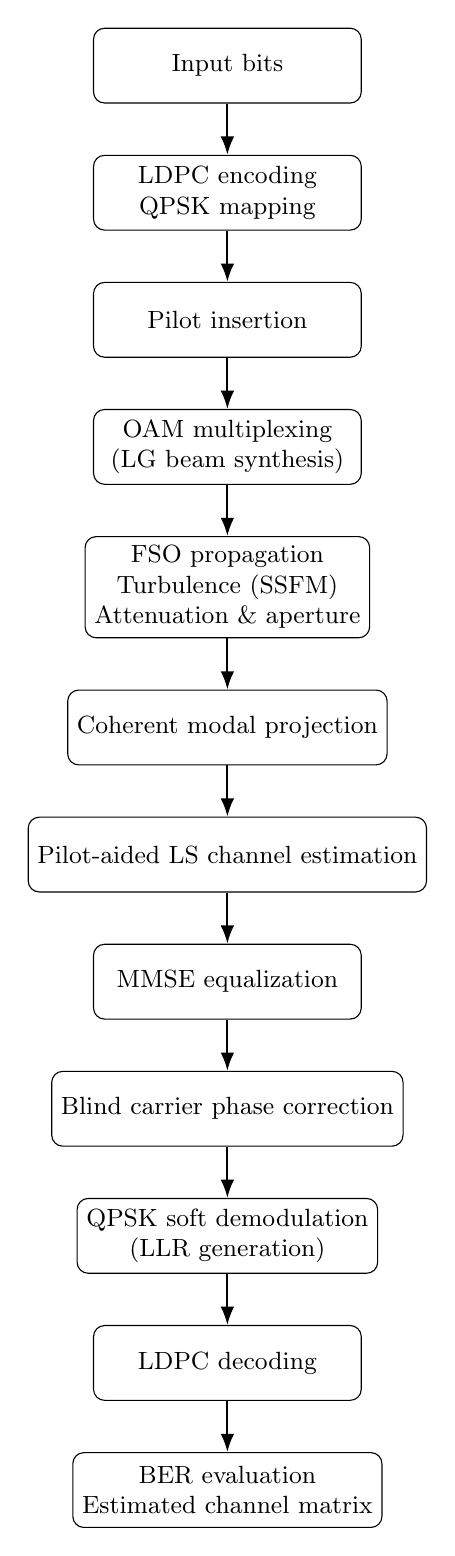
\begin{tikzpicture}[
node distance=6.5mm,
block/.style={
draw,
rounded corners,
align=center,
minimum width=3.4cm,
minimum height=0.95cm,
font=\small
},
line/.style={-Latex, thick}
]

\node[block] (bits) {Input bits};

\node[block, below=of bits] (enc)
{LDPC encoding\\QPSK mapping};

\node[block, below=of enc] (pilot)
{Pilot insertion};

\node[block, below=of pilot] (oam)
{OAM multiplexing\\(LG beam synthesis)};

\node[block, below=of oam] (channel)
{FSO propagation\\Turbulence (SSFM)\\Attenuation \& aperture};

\node[block, below=of channel] (proj)
{Coherent modal projection};

\node[block, below=of proj] (ls)
{Pilot-aided LS channel estimation};

\node[block, below=of ls] (mmse)
{MMSE equalization};

\node[block, below=of mmse] (phase)
{Blind carrier phase correction};

\node[block, below=of phase] (demod)
{QPSK soft demodulation\\(LLR generation)};

\node[block, below=of demod] (ldpc)
{LDPC decoding};

\node[block, below=of ldpc] (ber)
{BER evaluation\\Estimated channel matrix};

% arrows
\draw[line] (bits) -- (enc);
\draw[line] (enc) -- (pilot);
\draw[line] (pilot) -- (oam);
\draw[line] (oam) -- (channel);
\draw[line] (channel) -- (proj);
\draw[line] (proj) -- (ls);
\draw[line] (ls) -- (mmse);
\draw[line] (mmse) -- (phase);
\draw[line] (phase) -- (demod);
\draw[line] (demod) -- (ldpc);
\draw[line] (ldpc) -- (ber);

\end{tikzpicture}
\label{fig:vertical_chain}
\end{figure}



\end{document}